%%% CV page
\begin{curriculumvitae}

% 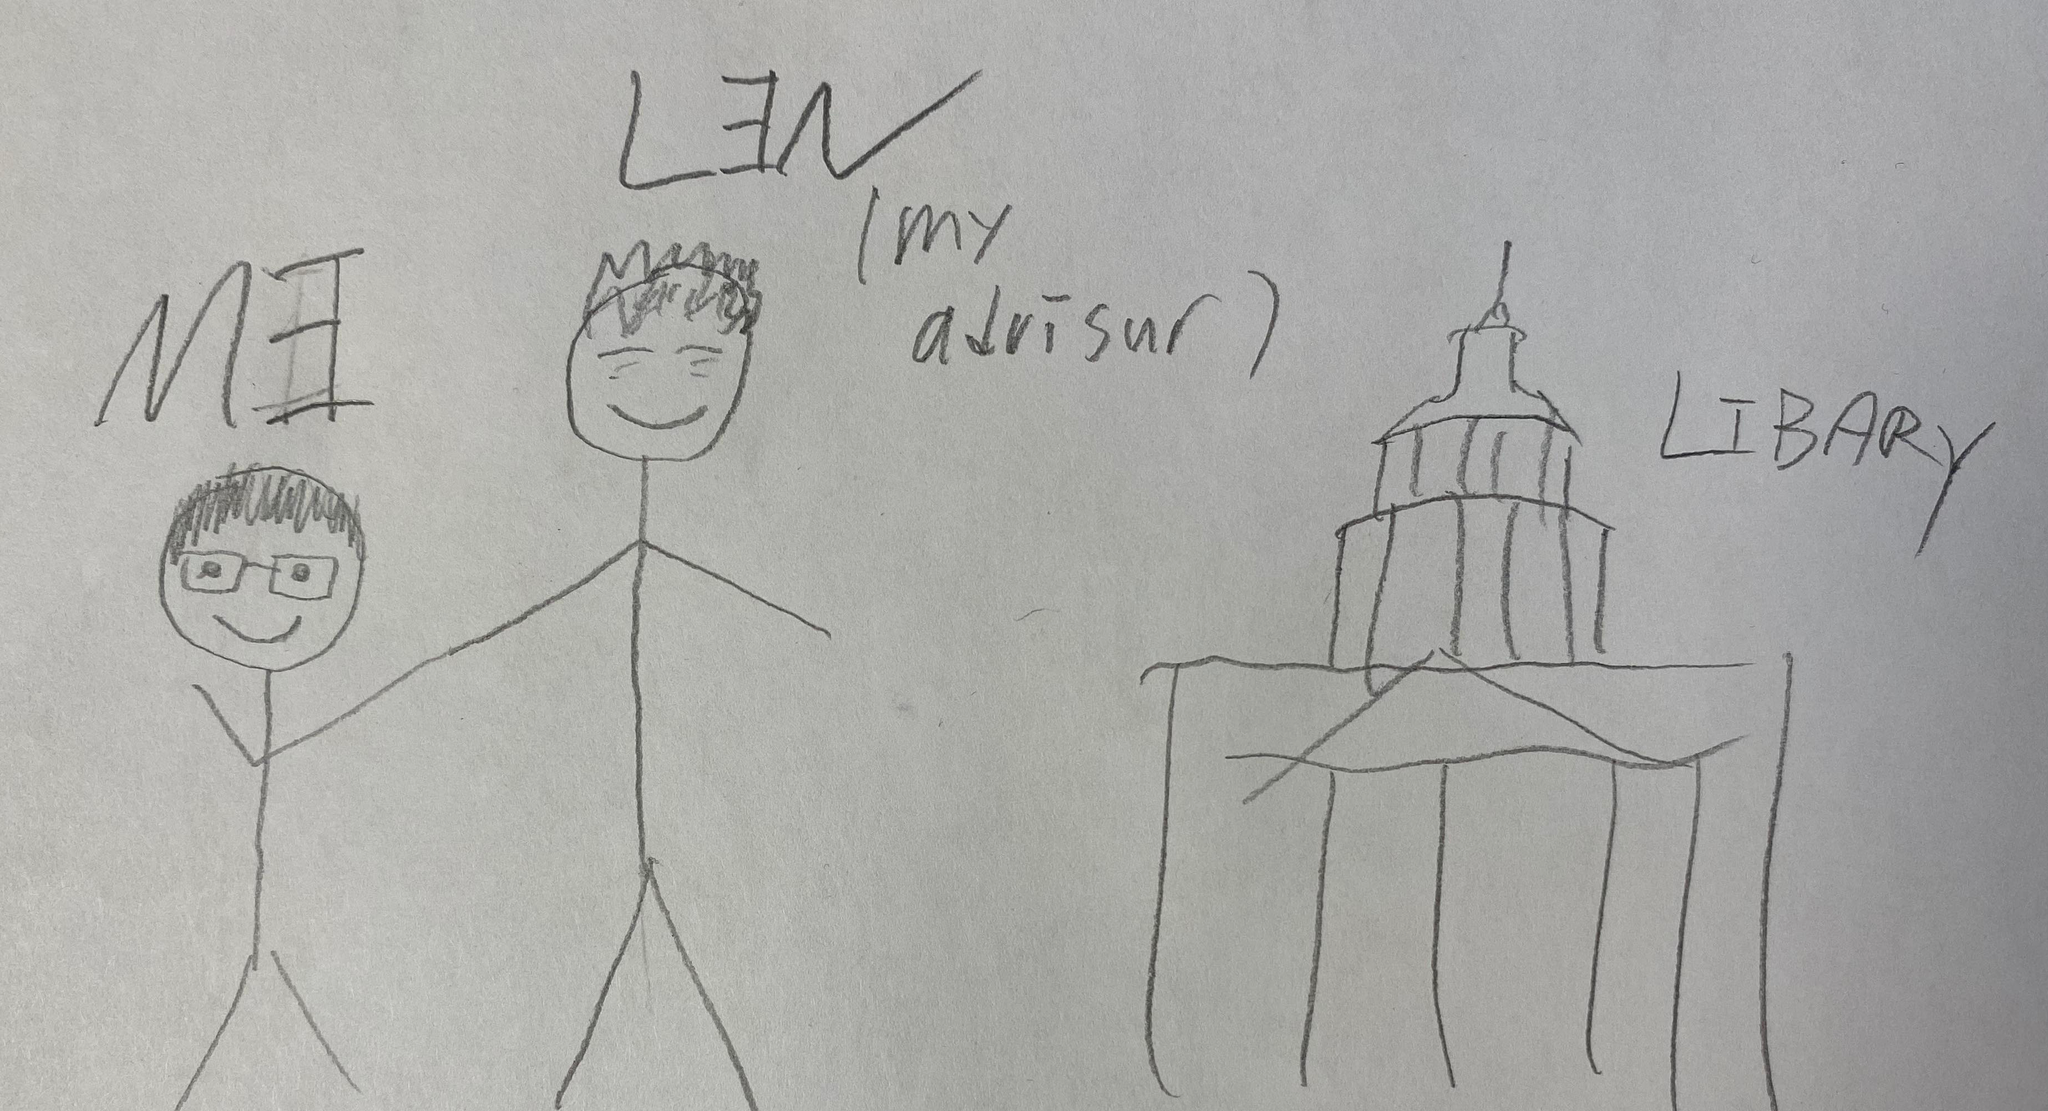
\includegraphics[width=\textwidth]{preamble/biosketch.png}

%In one to three paragraphs, provide some basic facts about your scholarly life and career, without including personal data such as birth date. The information listed in this section should be limited to professional experience that is related to the field of the dissertation. These include the colleges and universities attended, the major fields of study at each, and the degrees and academic honors awarded. If you have relevant professional experience such as employment in your career field, you may describe it briefly. Follow this with a description of your work at the University of Rochester, including dates of residence, graduate programs pursued, name(s) of advisor(s), and all university appointments (e.g. fellowships, scholarships, research and teaching assistantships or traineeships). Do not include a complete scientific curriculum vitae or professional resume. Do not include future plans or employment.
Lane Lawley was born in Birmingham, Alabama, U.S.A. He was awarded his B.S. in Computer Science, \textit{magna cum laude}, by the Rochester Institute of Technology in 2015. He was then employed by Google until he began his doctoral studies at the University of Rochester, advised by Professor Lenhart Schubert, in 2017. In 2019, the University of Rochester awarded him his M.S. in Computer Science. In 2017 and 2018, he was awarded an NSF Research Traineeship.

%Follow this narrative with a reference list of all works published or in review for publication during your time at the University, including content or results from the dissertation that have been published in full or in part. This listing may include publications mentioned on the Contributors and Funding Sources page. See that section below on including previously published articles as chapters in the dissertation.

%Lane Lawley, Gene Louis Kim, and Lenhart Schubert. Towards natural language story understanding with rich logical schemas. In Proceedings of the Sixth Workshop on Natural Language and Computer Science, pages 11–22, Gothenburg, Sweden, May 2019. Association for Computational Linguistics.

He produced the following publications during his doctoral studies.

\begin{itemize}
    \item \textbf{Lane Lawley}, Gene Louis Kim, and Lenhart Schubert. \href{https://aclanthology.org/W19-1102/}{Towards natural language story understanding with rich logical schemas.} In \textit{Proceedings of the Sixth Workshop on Natural Language and Computer Science}, pages 11–22, Gothenburg, Sweden, May 2019. Association for Computational Linguistics.
    \item \textbf{Lane Lawley}, Benjamin Kuehnert, and Lenhart Schubert. \href{https://aclanthology.org/2021.naloma-1.1}{Learning general event schemas with episodic logic.} In \textit{Proceedings of the 1st and 2nd Workshops on Natural Logic Meets Machine Learning (NALOMA)}, pages 1–6, Groningen, the Netherlands (online), June 2021. Association for Computational Linguistics.
    \item \textbf{Lane Lawley}, Will Frey, Patrick Mullen, and Alexander D. Wissner-Gross. \href{https://doi.org/10.1177/1548512921996828}{Joint sparsity-biased variational graph autoencoders.} \textit{The Journal of Defense Modeling and Simulation}, 18(3):239–246, March 2021.
    \item Erin Gibson and \textbf{Lane Lawley}. \href{https://doi.org/10.32473/flairs.v35i.130703}{Language-model-based parsing and English generation for unscoped episodic logical forms.} In \textit{the International FLAIRS Conference Proceedings}, volume 35, May 2022.
    \item \textbf{Lane Lawley} and Lenhart Schubert. \href{https://aclanthology.org/2022.acl-srw.25}{Mining logical event schemas from pre-trained language models.} In \textit{Proceedings of the 60th Annual Meeting of the Association for Computational Linguistics: Student Research Workshop}, pages 332–345, Dublin, Ireland, May 2022. Association for Computational Linguistics.
    \item \textbf{Lane Lawley} and Lenhart Schubert. \href{https://aclanthology.org/2022.distcurate-1.3}{Logical story representations via FrameNet + semantic parsing.} In \textit{Proceedings of the Workshop on Dimensions of Meaning: Distributional and Curated Semantics (DistCurate 2022)}, pages 19–23, Seattle, Washington, July 2022. Association for Computational Linguistics.
\end{itemize}

\end{curriculumvitae}